\documentclass[11pt]{book}
\usepackage{fontspec}
\setmainfont{TeX Gyre Pagella}
\usepackage[margin=1in]{geometry}
\usepackage{xcolor}
\usepackage{tikz}
\usetikzlibrary{arrows.meta}
\usepackage{amssymb}
\usepackage{enumitem}
\usepackage{titlesec}

\titleformat{\chapter}[display]{\bfseries\Large}{Sproll 03}{0.5em}{\Huge}
\titleformat{\section}{\bfseries\large}{\thesection}{0.6em}{}

\newenvironment{algorithmproc}[1]{%
\vspace{0.6em}\noindent\rule{\linewidth}{0.6pt}\\[0.2em]\textbf{How to Tell: #1}\\[0.3em]}%
{\\[0.2em]\noindent\rule{\linewidth}{0.6pt}\vspace{0.6em}}

\newenvironment{practicenow}{%
\vspace{0.6em}\noindent\rule{\linewidth}{0.6pt}\\[0.2em]\textbf{Practice Now}\\[0.3em]}%
{\\[0.2em]\noindent\rule{\linewidth}{0.6pt}\vspace{0.6em}}

\newenvironment{exercisebox}[1]{%
\vspace{0.8em}\noindent\rule{\linewidth}{0.6pt}\\[0.2em]\textbf{Exercises: #1}\\[0.3em]%
\begin{enumerate}[label=\arabic*., itemsep=0.4em]}%
{\end{enumerate}\noindent\rule{\linewidth}{0.6pt}\vspace{0.6em}}

\newenvironment{trythis}{%
\vspace{0.6em}\noindent\rule{\linewidth}{0.6pt}\\[0.2em]\textbf{Try This}\\[0.3em]}%
{\\[0.2em]\noindent\rule{\linewidth}{0.6pt}\vspace{0.6em}}

\newenvironment{summarybox}{%
\vspace{0.6em}\noindent\rule{\linewidth}{0.6pt}\\[0.2em]\textbf{What We Learned}\\[0.3em]}%
{\\[0.2em]\noindent\rule{\linewidth}{0.6pt}\vspace{0.6em}}

\begin{document}
\begin{titlepage}
\centering
\vspace*{1.4in}
{\Huge \textbf{SPROLL 03}}\\[0.5in]
{\huge Play It Again}\\[0.8in]
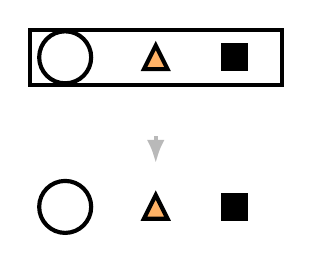
\begin{tikzpicture}
\draw[line width=1.5pt] (-1.6,0.55) rectangle (1.6,1.25);
\draw[line width=1.5pt] (-1.15,0.9) circle (0.13in);
\draw[fill=orange!60, line width=1.5pt] (-0.15,0.75) -- (0,1.05) -- (0.15,0.75) -- cycle;
\draw[fill=black, line width=1.5pt] (0.85,0.75) rectangle (1.15,1.05);
\draw[-{Latex[length=3mm]}, line width=1.6pt, gray!55] (0,-0.1) -- (0,-0.45);
\draw[line width=1.5pt] (-1.15,-1.0) circle (0.13in);
\draw[fill=orange!60, line width=1.5pt] (-0.15,-1.15) -- (0,-0.85) -- (0.15,-1.15) -- cycle;
\draw[fill=black, line width=1.5pt] (0.85,-1.15) rectangle (1.15,-0.85);
\end{tikzpicture}\\[0.5in]
{\Large The Sproll Curriculum}\\[0.2in]
{\large Cycle I: Pops --- Things, Differences, and Counting}
\end{titlepage}

\tableofcontents

\chapter*{Before You Begin}
\addcontentsline{toc}{chapter}{Before You Begin}

Sproll 02 showed that a picture, on its own, can lose information a kept record would have preserved, in particular, the order in which things happened. This workbook asks the next natural question. If a record really does preserve everything that happened, could you use it to actually rebuild the events themselves, not just read a description of them? And if you did, would you always get back exactly the same result?

This turns out to be one of the most important ideas in this entire curriculum, and it is the first place this series asks you to trust something the way mathematicians trust a proof: not because someone told you it was true, but because you can check it yourself, every single time, and get the same answer.

\chapter{A Record You Can Follow Again}

\section{Following Steps in Order}

Think about a recipe. A recipe is a kind of record: a list of steps, in a specific order, describing choices someone else already made, this ingredient, then that one, mixed in this way, baked for this long. A recipe is not just a description of a cake that already exists. It is written so that anyone who follows it, step by step, in the order given, can produce that same cake themselves.

This is exactly the idea this workbook calls \textbf{replay}: taking a record of what happened, and actually redoing each step, in order, to rebuild the result the record describes.

\begin{center}
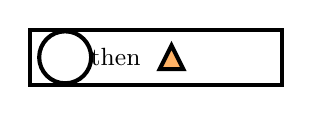
\begin{tikzpicture}
\draw[line width=1.5pt] (-1.6,0.55) rectangle (1.6,1.25);
\draw[line width=1.5pt] (-1.15,0.9) circle (0.13in);
\node[right] at (-0.95,0.9) {\small then};
\draw[fill=orange!60, line width=1.5pt] (0.05,0.75) -- (0.2,1.05) -- (0.35,0.75) -- cycle;
\end{tikzpicture}
\end{center}

Recall the ledger strip from Sproll 02. This particular record says: circle, then triangle. To replay it, you would not simply look at the strip and imagine the result. You would actually choose the circle, and then actually choose the triangle, in that order, and see what you end up with. Following a record this way is different from just reading it; it is repeating the choices themselves.

\begin{algorithmproc}{How to Replay a Record}
To replay a record, work through it one entry at a time, in the exact order it is written. For each entry, perform the choice it describes before moving to the next entry. Do not skip ahead, and do not reorder the steps, even if a later step seems like it could come first. The record's order is the point.
\end{algorithmproc}

\begin{practicenow}
Find a short set of instructions you can actually follow, a simple recipe, a paper airplane pattern, the setup steps for a game. Follow it exactly, in order, and see whether you get the result it promises.
\end{practicenow}

\begin{exercisebox}{Section 1.1}
\item Explain, in your own words, the difference between reading a record and replaying a record.
\item Describe a record from your own life (a recipe, a set of directions, a list of dance steps) that is specifically meant to be replayed by someone else, not just read.
\item Why do you think the order matters so much when replaying a record, even if every individual step, on its own, seems simple?
\end{exercisebox}

\chapter{Does Replaying Always Give the Same Result?}

\section{The Promise a Record Makes}

Here is the important claim this workbook wants you to test for yourself, not just believe because it is written down. If you replay the exact same record, following the exact same steps in the exact same order, starting from the exact same conditions, you should get the exact same result every single time. Not almost the same. The same.

Think about instructions for building something out of building blocks, following a numbered diagram, one piece at a time. If you follow the diagram correctly, step 1, then step 2, then step 3, and so on, you will end up with the same finished model as anyone else who followed the same diagram correctly. This is true even if you build it on a Tuesday and your friend builds it on a Saturday, even if you build it in a different room, even if years pass in between. The record does not care about any of that. It only cares whether the steps were followed, in order.

\begin{algorithmproc}{Testing a Record's Promise}
To test whether a record truly determines its result, replay it twice, as carefully and exactly as you can both times. If you get the same result both times, the record has kept its promise. If you get a different result, look closely: either the record itself was incomplete or unclear about some step, or one of your two attempts did not actually follow it exactly. A record that is complete and followed exactly always gives back the same result.
\end{algorithmproc}

\begin{trythis}
Pick a short, exact set of folding instructions (a simple paper airplane or origami shape works well). Follow the instructions once, and set the result aside without looking at it again. Follow the exact same instructions a second time, from a fresh piece of paper. Compare your two results. Are they the same shape?
\end{trythis}

\begin{exercisebox}{Section 2.1}
\item If two people follow the exact same, clearly written instructions and end up with two different results, what are the possible explanations? List at least two.
\item Explain why ``the exact same steps, in the exact same order'' is a stronger claim than just ``roughly the same steps.''
\item Challenge: can you think of a situation where a record looks complete, but actually leaves out a detail that could cause two people following it to get slightly different results? Describe it.
\end{exercisebox}

\chapter{Why Replay Is Like a Proof}

\section{Don't Tell Me, Show Me}

Suppose a friend tells you they built an enormous tower out of blocks, twenty stories tall, and it did not fall down. You could simply believe them. Or, if they kept a careful record of exactly how they built it, which block went where and in what order, you could follow that record yourself and see whether the same tower actually results, and whether it actually stands.

This is the heart of what this workbook calls the ``play it again'' idea, and it is close to what mathematicians and scientists mean by a proof. A proof is not simply a strong claim, stated confidently. It is a record, written clearly enough that someone else can follow every step themselves and reach the same conclusion, without having to take the original claim on faith. ``Don't tell me what happened. Show me the record, and let me play it again.''

This is a genuinely different kind of trust from trusting a person's word. You are not trusting that your friend is honest, or has a good memory, or is not exaggerating. You are trusting that the steps, followed exactly, lead to the result, and you can check that for yourself, as many times as you like, without needing to trust anyone at all.

\begin{summarybox}
Replay means following a record's steps in order to rebuild what it describes, rather than only reading about it. A complete, clearly written record, followed exactly, gives back the same result every time it is replayed, no matter who replays it or when. This is why a good record can settle a disagreement that a person's word alone cannot: instead of asking someone to trust a claim, you can hand them the record and let them check it themselves.
\end{summarybox}

\begin{exercisebox}{Section 3.1}
\item Describe a disagreement between two people that could be settled by a kept record, rather than by one person simply insisting they are right.
\item Explain in your own words why ``you can check it yourself'' is a stronger kind of proof than ``someone you trust said so.''
\item Challenge: think of a claim you have heard that would be hard to check yourself, even with a record, because the record itself would be difficult or impossible to keep. What makes that case different from the recipe and building-block examples in this workbook?
\end{exercisebox}

\chapter*{Looking Ahead}
\addcontentsline{toc}{chapter}{Looking Ahead}

Every record in this workbook so far has described choices that were made, this shape, then that shape. But a record could also describe something else: a choice that was considered and specifically \emph{not} made. Is that kind of entry, a choice that did not happen but is still written down on purpose, the same as simply leaving it out of the record entirely? That question, and why the answer matters more than it might seem, is the subject of the next workbook, Sproll 04: Not This Way.

\chapter*{For Parents and Teachers}
\addcontentsline{toc}{chapter}{For Parents and Teachers}

This workbook introduces replay and, with it, the child's first encounter with a distinguishing feature of mathematical proof: a claim's trustworthiness resting on the ability of anyone to check it independently by following the same steps, rather than on the reliability of whoever states the claim. The underlying formal guarantee, that replaying a deterministic record twice yields identical results, is not asserted here as a simplification; it is a genuine, provable property of the historical-construction system this curriculum builds toward, stated informally here and given a precise formal treatment (a Replay Determinism proposition) in the technical companion material for this curriculum.

Chapter 2's ``testing a record's promise'' section is deliberately framed as an experiment the child performs, not a fact they are told, consistent with this curriculum's broader commitment to letting a child discover a mathematical fact by direct construction wherever possible, rather than asserting it and asking for trust. Chapter 3 connects this directly to the everyday meaning of settling a disagreement by checking rather than by appeal to authority, which is offered as an accessible entry point to a formal idea (verifiability) this curriculum returns to with more precision in its Broken Maps material later in the series.

\end{document}
